\documentclass{article}
\usepackage{graphicx}
\usepackage{indentfirst}
\usepackage[hidelinks]{hyperref}
\usepackage{url}
\usepackage{multicol}
\usepackage[a4paper, total={5.5in, 8.5in}]{geometry}

\title{IFT712 - Rapport de projet de session}

\author{Tom SARTORI \and Louis-Vincent CAPELLI \and Alexandre THEISSE}

\date{\today}


\begin{document}
\maketitle
\newpage

\tableofcontents
\newpage

\section{Contexte}
Ce projet a été réalisé dans le cadre du cours \textbf{IFT712 - Techniques d'apprentissage} de
l'université de Sherbrooke. Il consiste à utiliser des méthodes de classification
de la bibliothèque \textit{scikit-learn} sur une base de données Kaggle.

Le lien du GitHub associé est le suivant : \url{https://github.com/BigBaz54/leaf_classification}


\section{Présentation de la base de données}
Nous avons choisi la base de données \textit{Leaf Classification} \cite{leafKaggle} 
comme conseillé dans le sujet du projet. Cette base de données contient des images de feuilles
de différentes espèces. L'objectif est de prédire l'espèce d'une feuille à partir de ses
caractéristiques (features) qui incluent 64 mesures représentant le contour de la feuille (margin) 
\cite{leafMargin}, 64 mesures représentant la forme de la feuille (shape) et 64 mesures
représentant la texture de la feuille (texture). 

La base de données contient 990 feuilles pour lesquelles l'espèce est connue et dont l'image
est disponible. Les feuilles appartenant à 99 espèces différentes, il y a donc 10 feuilles
par espèce.

\section{Préparation des données}
Afin de pouvoir utiliser les méthodes de classification de \textit{scikit-learn}, nous avons
dû préparer les données. 

Les features ont été séparées des labels afin de pouvoir entraîner les modèles et
ensuite évaluer leur performance en comparant les labels prédits avec les labels réels.

Nous avons également formé un ensemble d'entraînement et un ensemble de test à partir 
de l'ensemble d'entraînement initial fourni par Kaggle. Nous n'avons pas pu utiliser
l'ensemble de test fourni par Kaggle car il ne contenait pas les labels correspondants
aux échantillons.

Pour ce faire, nous avons utilisé la classe
\textit{StratifiedShuffleSplit} \cite{SSS} de \textit{scikit-learn} qui permet de séparer les données
en conservant la proportion de chaque classe dans chaque ensemble.

\newpage
\section{Classification sur les features}
Cette approche est celle attendue au vu de la base de données : elle consiste à prédire l'espèce
d'une feuille à partir de ses caractéristiques. Nous avons donc utilisé les 192 features
(margin, shape et texture) pour entraîner nos modèles.

\subsection{Sélection des features}
La première étape a été de sélectionner un sous-ensemble pertinent de features. 

D'après notre
compréhension de la base de données, elle contient 3 groupes de 64 features qui représentent
respectivement le contour, la forme et la texture de la feuille. Nous avons donc considéré
que chacun de ces 3 groupes devait être utilisé comme un tout représentant
une seule et même information et que ce n'était pas pertinent
de sélectionner des features individuellement au sein de ces groupes.

Également, nous avions l'intuition que ces 3 informations étaient complémentaires et qu'elles
ne présentaient pas de redondance. Nous avons tout de même, pour s'en assurer, entraîné des
modèles sur différents sous-ensembles des 3 groupes de features et comparé leurs performances. 
Ci-dessous, les résultats obtenus avec un SVC \cite{SVC} :

\begin{figure}[h]
    \centering
    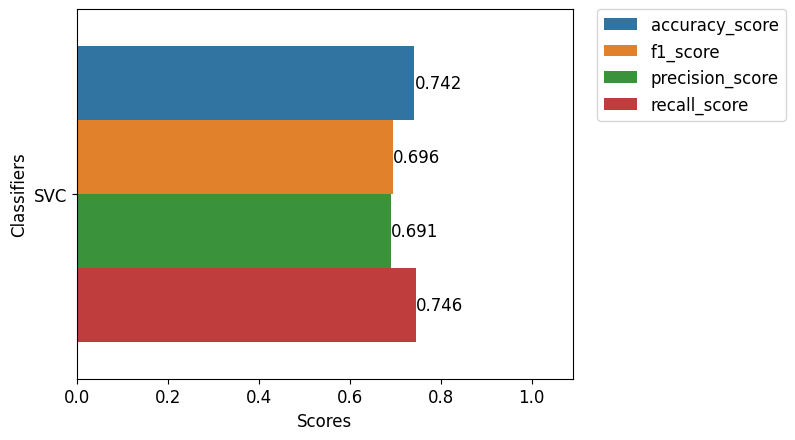
\includegraphics[width=0.8\textwidth]{img/svc_perfs_without_margin.png}
    \caption{Performances d'un SVC sur les 128 features de shape et texture}
\end{figure}

\begin{figure}[h]
    \centering
    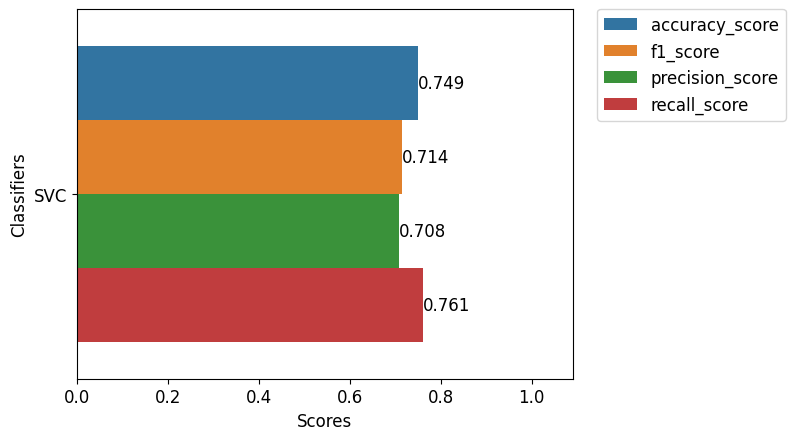
\includegraphics[width=0.8\textwidth]{img/svc_perfs_without_texture.png}
    \caption{Performances d'un SVC sur les 128 features de margin et shape}
\end{figure}

\begin{figure}[h]
    \centering
    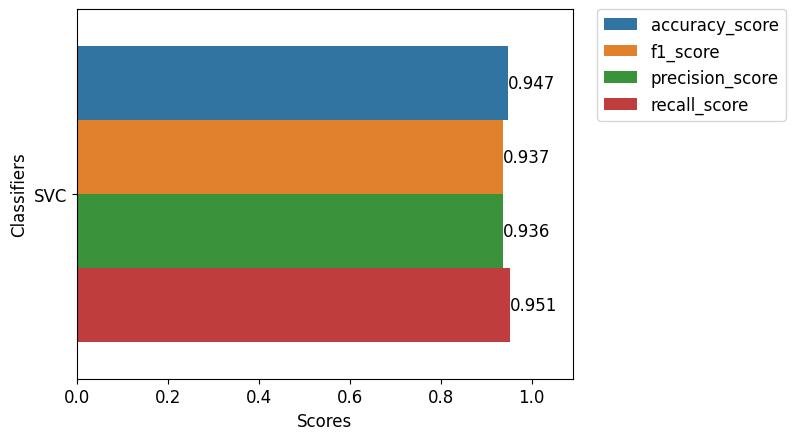
\includegraphics[width=0.8\textwidth]{img/svc_perfs_all_data.png}
    \caption{Performances d'un SVC sur l'ensemble des 192 features}
\end{figure}
\newpage

Les résultats obtenus confirment notre intuition : les 3 groupes de features sont complémentaires
et fournissent des meilleurs résultats lorsqu'ils sont utilisés ensemble. Nous avons donc
décidé pour la suite de l'étude de considérer les 192 features à notre disposition.

\newpage
\subsection{Classification}

\subsubsection{Modèles utilisés}
Nous avons utilisé les modèles suivants pour la classification :
\begin{itemize}
    \item \textit{DecisionTreeClassifier} \cite{DTC} : arbre de décision
    \item \textit{RandomForestClassifier} \cite{RFC} : forêt aléatoire
    \item \textit{BaggingClassifier} \cite{BC} : agrégation de modèles
    \item \textit{LogisticRegression} \cite{LR} : régression logistique
    \item \textit{SVC} \cite{SVC} : machine à vecteurs de support
    \item \textit{GaussianNB} \cite{GNB} : modèle naïf bayésien gaussien
    \item \textit{SGDClassifier} \cite{SGD} : descente de gradient stochastique
    \item \textit{KNeighborsClassifier} \cite{KNN} : k plus proches voisins
    \item \textit{GradientBoostingClassifier} \cite{GNB} : gradient boosting
    \item \textit{MLPClassifier} \cite{MLP} : perceptron multicouche
    \item \textit{AdaBoostClassifier} \cite{ABC} : AdaBoost
\end{itemize}

Nous avons séléctionné ces modèles pour leur diversité, en effet ils utilisent
des approches différentes pour la classification : certains sont des modèles linéaires,
d'autres sont des modèles non-linéaires, certains sont des modèles à base de règles,
d'autres sont des modèles à base de probabilités, etc. 

Le but était de maximiser nos chances de trouver un modèle performant sur cette
base de données en utilisant des modèles assez différents les uns des autres.

\newpage
\subsubsection{Cross-validation}
Nous avons commencé par entraîner les modèles sur l'ensemble d'entraînement pour
avoir un premier aperçu de leurs performances et une base de comparaison.
\\\\
Voici les résultats obtenus :

\begin{figure}[h]
    \centering
    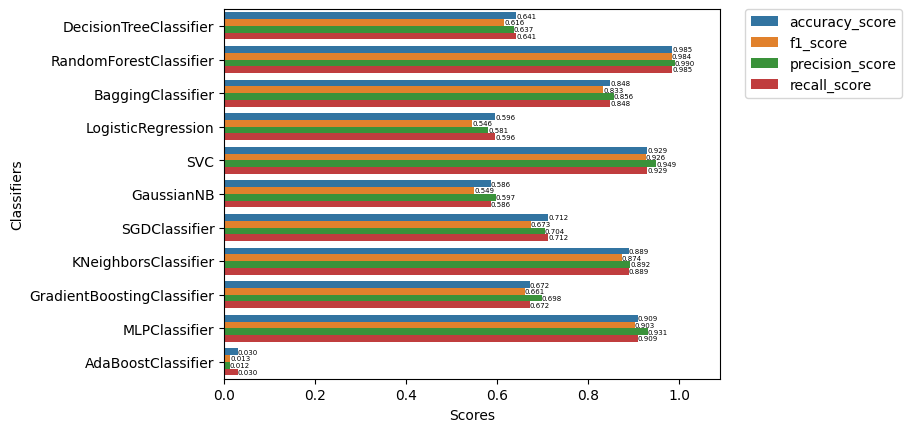
\includegraphics[width=1.2\textwidth]{img/all_perfs_without_cv.png}
    \caption{Performances des différents modèles sur tout l'ensemble d'entraînement}
\end{figure}


Nous avons ensuite utilisé la fonction \textit{cross\_validate} \cite{CV} de \textit{scikit-learn}
qui permet de faire une validation croisée avec un nombre de folds donné et d'utiliser 
le multi-threading pour accélérer le processus. Cette fonction utilise aussi la 
stratégie de \textit{StratifiedShuffleSplit} \cite{SSS} pour séparer les données en
folds tout en conservant la proportion de chaque classe dans chaque fold.

Nous avons donc établi un nombre de folds maximal qui s'assure que chaque fold 
contient au moins un représentant de chaque classe.
\newpage
Voici les résultats obtenus :

\begin{figure}[h]
    \centering
    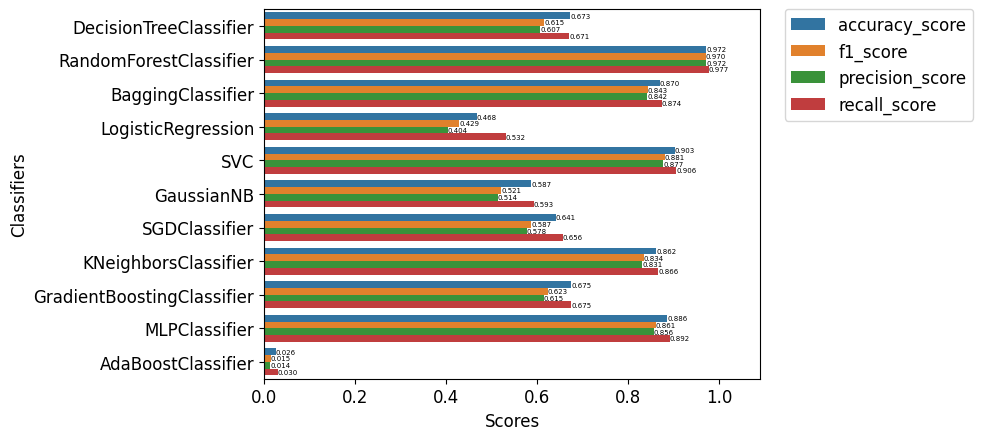
\includegraphics[width=1.2\textwidth]{img/all_perfs_with_cv.png}
    \caption{Performances des différents modèles avec une validation croisée à 10 folds}
\end{figure}


Les résultats obtenus sont similaires à ceux obtenus sans validation croisée, et sont
même légèrement moins bons pour certains modèles. Cela peut s'expliquer par le fait
que la base de données est assez petite (10 représentants par classe en tout, donc
encore moins dans les données d'entraînement) et que la validation croisée réduit encore
la taille de l'ensemble d'entraînement. 

Dans ce cas, les modèles sont entraînés à plusieurs reprises
sur des ensembles d'entraînement qui ne contiennent qu'un ou deux représentants de chaque classe,
et ont donc plus de difficultés à généraliser. Cet effet est visible par exemple sur le 
graphique suivant, qui montre la précision obtenue pour les différents folds de la validation
croisée d'un modèle de régression logistique :

\begin{figure}[h]
    \centering
    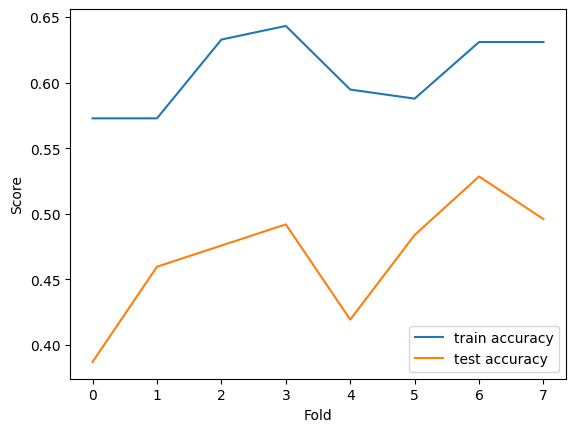
\includegraphics[width=0.6\textwidth]{img/folds_perfs_logreg.png}
    \caption{Performances d'un modèle de régression logistique sur les différents folds de la validation croisée}
\end{figure}
\newpage

On constate également sur le graphique suivant que la précision de certains modèles
(ici une forêt aléatoire) n'augmente
pas linéairement avec le nombre de représentants de chaque classe dans l'ensemble d'entraînement
et qu'il serait donc judicieux d'inclure au minimum 3 représentants de chaque classe dans chaque
fold de la validation croisée :

\begin{figure}[h]
    \centering
    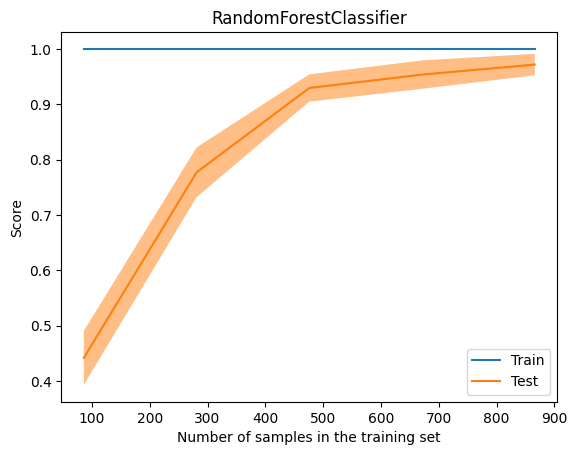
\includegraphics[width=0.6\textwidth]{img/perf_vs_samples_rf.png}
    \caption{Performances d'un modèle de régression logistique sur les différents folds de la validation croisée}
\end{figure}

Nous avons donc décidé, pour réduire cet effet, de n'utiliser que 2 ou 3 folds pour la
validation croisée pour la suite de l'étude.

\newpage
\subsubsection{Recherche d'hyperparamètres}
Jusqu'à présent, nous avons utilisé les hyperparamètres par défaut des \\modèles. Pour améliorer
leurs performances, il fallait donc les optimiser. Pour ce faire, nous avons utilisé la fonction
\textit{GridSearchCV} \cite{GSCV} de \textit{scikit-learn} qui permet de faire une recherche
d'hyperparamètres par validation croisée. La fonction \textit{GridSearchCV} permet de spécifier
une grille de valeurs pour chaque hyperparamètre et va tester toutes les combinaisons possibles
pour trouver celle qui donne les meilleurs résultats. C'est une méthode d'exploration exhaustive
qui est donc assez coûteuse en calcul.

Nous avons choisi les hyperparamètres à optimiser en fonction de la documentation des modèles
et les valeurs à tester sont le fruit de plusieurs essais au cours desquels nous avons
raffiné la grille de recherche pour s'assurer de ne pas passer à côté de valeurs intéressantes.

Les grilles de recherche utilisées sont disponibles dans le notebook \\
\textit{features\_hyperparam\_search.ipynb}, voici les valeurs optimales obtenues pour
chaque modèle :

\begin{footnotesize}
\begin{multicols}{2}
\begin{itemize}
    \item \textit{DecisionTreeClassifier} :
    \begin{itemize}
        \item \textit{criterion} : gini
        \item \textit{max\_depth} : None
        \item \textit{max\_features} : sqrt
        \item \textit{min\_samples\_leaf} : 1
        \item \textit{min\_samples\_split} : 5
        \item \textit{splitter} : best
    \end{itemize}
    \item \textit{RandomForestClassifier} :
    \begin{itemize}
        \item \textit{criterion} : gini
        \item \textit{max\_features} : log2
        \item \textit{min\_samples\_split} : 2
        \item \textit{n\_estimators} : 500
    \end{itemize}
    \item \textit{BaggingClassifier} :
    \begin{itemize}
        \item \textit{bootstrap} : False
        \item \textit{bootstrap\_features} : True
        \item \textit{max\_features} : 0.1
        \item \textit{max\_samples} : 0.5
        \item \textit{n\_estimators} : 100
    \end{itemize}
    \item \textit{SGDClassifier} :
    \begin{itemize}
        \item \textit{alpha} : 0.0001
        \item \textit{loss} : modified\_huber
        \item \textit{max\_iter} : 2000
        \item \textit{penalty} : l1
    \end{itemize}
    \item \textit{LogisticRegression} :
    \begin{itemize}
        \item \textit{C} : 1000
        \item \textit{max\_iter} : 100
        \item \textit{penalty} : l2
        \item \textit{solver} : liblinear
    \end{itemize}
    \item \textit{GaussianNB} :
    \begin{itemize}
        \item \textit{var\_smoothing} : 0.005
    \end{itemize}
    \item \textit{SVC} :
    \begin{itemize}
        \item \textit{C} : 50
        \item \textit{gamma} : scale
        \item \textit{kernel} : linear
    \end{itemize}
    \item \textit{KNeighborsClassifier} :
    \begin{itemize}
        \item \textit{algorithm} : auto
        \item \textit{leaf\_size} : 1
        \item \textit{n\_neighbors} : 1
        \item \textit{p} : 1
        \item \textit{weights} : distance
    \end{itemize}
    \item \textit{GradientBoostingClassifier} :
    \begin{itemize}
        \item \textit{learning\_rate} : 0.025
        \item \textit{max\_depth} : 2
        \item \textit{max\_features} : log2
        \item \textit{min\_samples\_split} : 10
        \item \textit{n\_estimators} : 500
    \end{itemize}
    \item \textit{MLPClassifier} :
    \begin{itemize}
        \item \textit{alpha} : 0.01
        \item \textit{hidden\_layer\_sizes} : (100,)
        \item \textit{learning\_rate} : adaptive
        \item \textit{max\_iter} : 500
        \item \textit{solver} : lbfgs
    \end{itemize}
    \item \textit{AdaBoostClassifier} :
    \begin{itemize}
        \item \textit{algorithm} : SAMME.R
        \item \textit{learning\_rate} : 0.01
        \item \textit{n\_estimators} : 500
    \end{itemize}
\end{itemize}
\end{multicols}
\end{footnotesize}

\subsection{Résultats}
Avec les hyperparamètres optimisés, et en utilisant une validation croisée à 2 folds,
voici les résultats obtenus :

\begin{figure}[h]
    \centering
    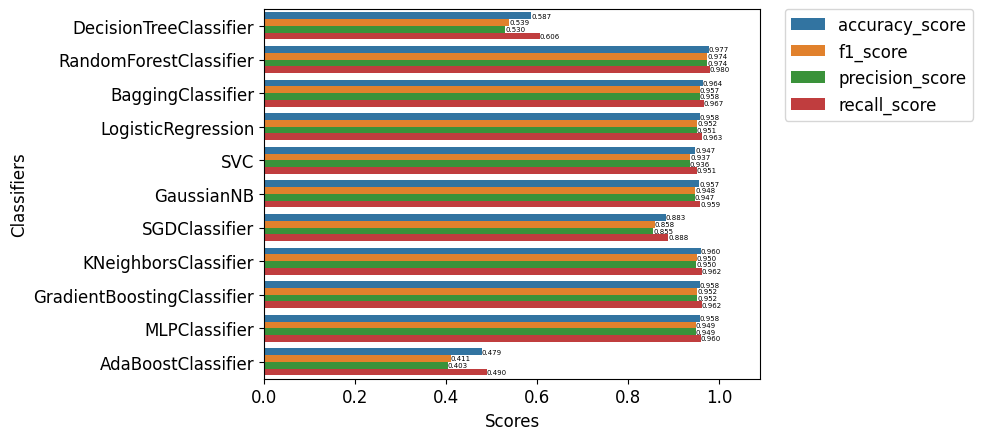
\includegraphics[width=1.2\textwidth]{img/all_perfs_with_cv_and_best_hp.png}
    \caption{Performances des différents modèles avec une validation croisée à 2 folds et des hyperparamètres optimisés}
\end{figure}

Les performances sont bien meilleures qu'avec les hyperparamètres par défaut pour certains
modèles, notamment LogisticRegression, GaussianNB, GradientBoostingClassifier
et AdaBoostClassifier.

\newpage
\section{Classification sur les images}
En plus de l'approche traditionnelle de classification sur les features, nous avons
décidé d'essayer une approche de classification sur les images. 

\subsection{Prétraitement des images}
Pour ce faire, nous avons
utilisé la bibliothèque \textit{Pandas} \cite{pandas} pour transformer les images en
tableaux de pixels.

Comme elles ne sont pas toutes de la même taille, nous avons dû les redimensionner
pour que chacune soit représentée par une vecteur de même dimension. Nous avons
essayé plusieurs manières,
mais celle que nous avons retenue est de déterminer la taille maximale des images
et de redimensionner toutes les images à cette taille en les centrant et en remplissant
les pixels manquants avec des pixels noirs. Cette méthode permet de conserver
la forme de la feuille et de ne pas les compresser afin de ne pas perdre d'information,
au niveau des contours notamment.

Nous avons enfin applati ces tableaux pour obtenir finalement un vecteur de features de taille
1778337.

Les images étant en noir et blanc, parmi les 256 valeurs possibles pour chaque pixel,
seules 2 sont utilisées : 0 pour le noir et 255 pour le blanc.

\begin{figure}[h]
    \centering
    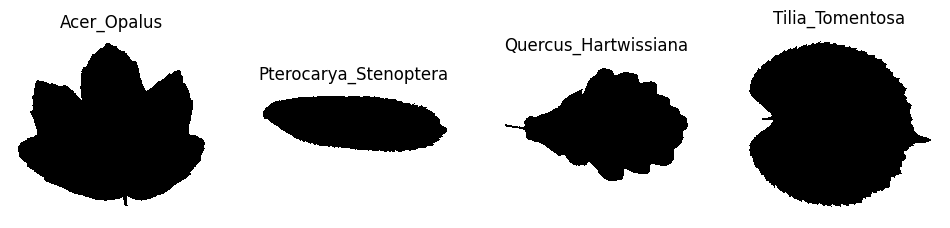
\includegraphics[width=0.9\textwidth]{img/img_examples.png}
    \caption{Exemples d'images de la base de données}
\end{figure}



L'approche que nous avons choisi pourrait poser problème car certaines feuilles se
retrouvent plus petites que d'autres dans les images finales, mais nous avons estimé
que cela ne devrait pas être le cas ici car même si les feuilles sont de tailles
différentes, au sein d'une même classe elles ont généralement des tailles similaires.

Cet effet pourrait donc même être bénéfique pour la classification et pourrait permettre
d'expliquer pourquoi le fait de redimensionner les images en les plaçant en haut à gauche
(notre première approche)
donne des résultats un peu moins bons que la méthode que nous avons finalement choisie.

\subsection{Classification}

\subsubsection{Modèles utilisés}

Nous avons utilisé les modèles suivants pour la classification basée sur les images :
\begin{itemize}
    \item \textit{RandomForestClassifier} \cite{RFC}
    \item \textit{KNeighborsClassifier} \cite{KNN}
\end{itemize}

Ce sont les 2 modèles parmi ceux que nous avons utilisés pour la classification sur les features
qui ont donné les meilleurs résultats et qui ont des temps d'entraînement assez faibles.

SVC, GradientBoostingClassifier et AdaBoostClassifier ont des temps \\
d'exécution raisonnables mais ont donné de moins bons résultats donc nous
ne les avons pas gardés car la recherche d'hyperparamètres était interminable.

\subsubsection{Cross-validation}
Nous avons utilisé la même stratégie de validation croisée que pour la classification
sur les features, c'est-à-dire une validation croisée à 2 folds afin de ne pas réduire
trop la taille de l'ensemble d'entraînement.

\subsubsection{Recherche d'hyperparamètres}

Nous avons utilisé la même stratégie de recherche d'hyperparamètres que pour la classification
sur les features, c'est-à-dire une recherche exhaustive avec la fonction \textit{GridSearchCV}
\cite{GSCV} de \textit{scikit-learn}. Les grilles de recherche utilisées sont disponibles
dans le notebook \textit{image\_hyperparam\_search.ipynb}, voici les valeurs optimales
obtenues pour chaque modèle :

\begin{small}
\begin{itemize}
    \item \textit{RandomForestClassifier} :
    \begin{itemize}
        \item \textit{criterion} : gini
        \item \textit{max\_features} : log2
        \item \textit{min\_samples\_split} : 2
        \item \textit{n\_estimators} : 500
    \end{itemize}
    \item \textit{KNeighborsClassifier} :
    \begin{itemize}
        \item \textit{algorithm} : TBD
        \item \textit{leaf\_size} : TBD
        \item \textit{n\_neighbors} : TBD
        \item \textit{p} : TBD
        \item \textit{weights} : TBD
    \end{itemize}
\end{itemize}
\end{small}

\subsection{Résultats}

Voici les résultats obtenus sans et avec optimisation des hyperparamètres :

\begin{figure}[h]
    \centering
    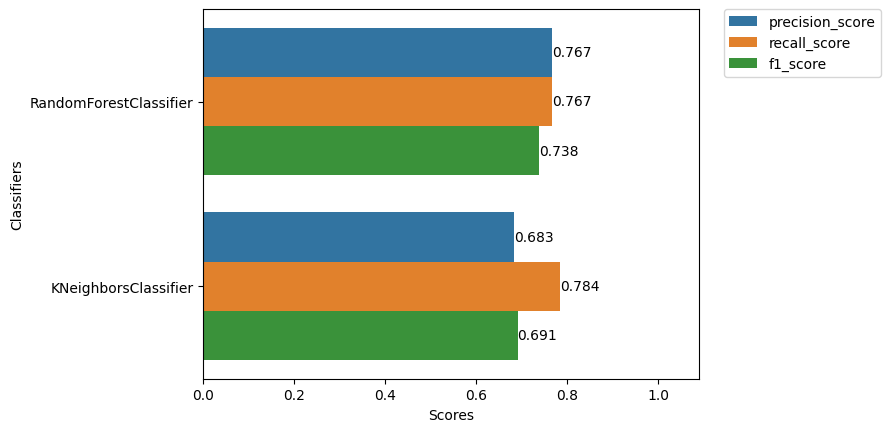
\includegraphics[width=0.8\textwidth]{img/img_perfs_without_cv_withou_hp.png}
    \caption{Performances des 2 modèles sans optimisation des hyperparamètres}
\end{figure}
\newpage

Nous avons également créé des fonctions permettant de visualiser les prédictions
des modèles sur les images de test. Voici quelques exemples : 

\begin{figure}[h]
    \centering
    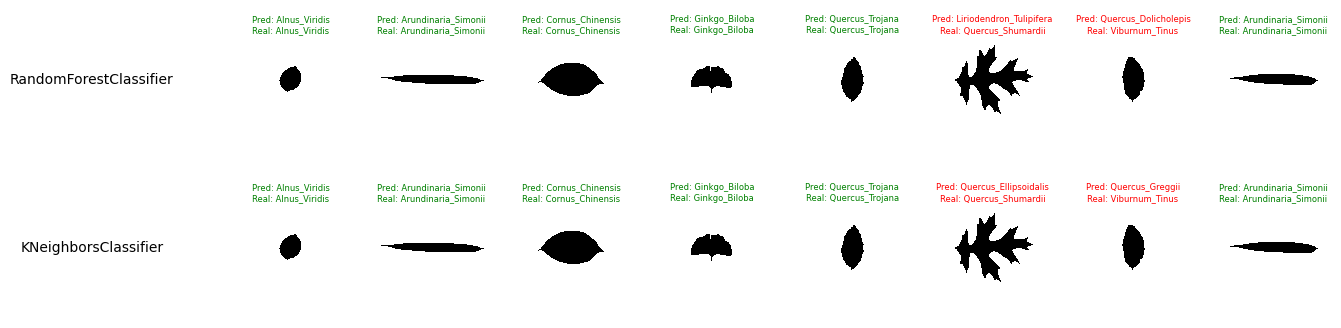
\includegraphics[width=1\textwidth]{img/img_preds.png}
    \caption{Exemples de prédictions des 2 modèles sur les images de test}
\end{figure}

\begin{figure}[h]
    \centering
    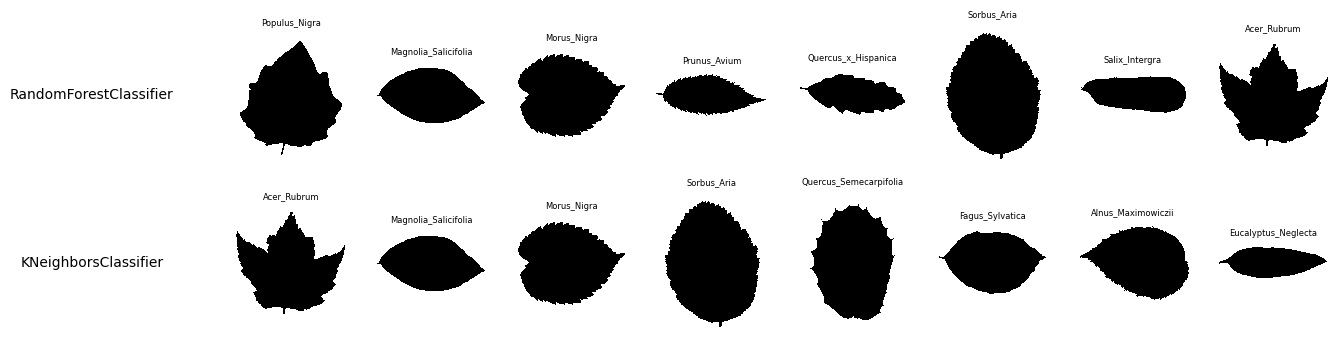
\includegraphics[width=1\textwidth]{img/img_worst_species.png}
    \caption{Classes présentant les moins bonnes performances}
\end{figure}

Nous sommes assez satisfaits des résultats obtenus, et même si les performances
sont moins bonnes que celles obtenues avec la classification sur les features,
nous avons trouvé intéressant de mettre en oeuvre cette approche alternative.

Les résultats moyens peuvent s'expliquer notamment par le nombre très bas
de représentants de chaque classe, par l'hétérogénéité des
tailles des images et par le fait que certaines images contiennent des feuilles
dans des orientations différentes, ce qui rend la généralisation impossible.

\begin{figure}[h]
    \centering
    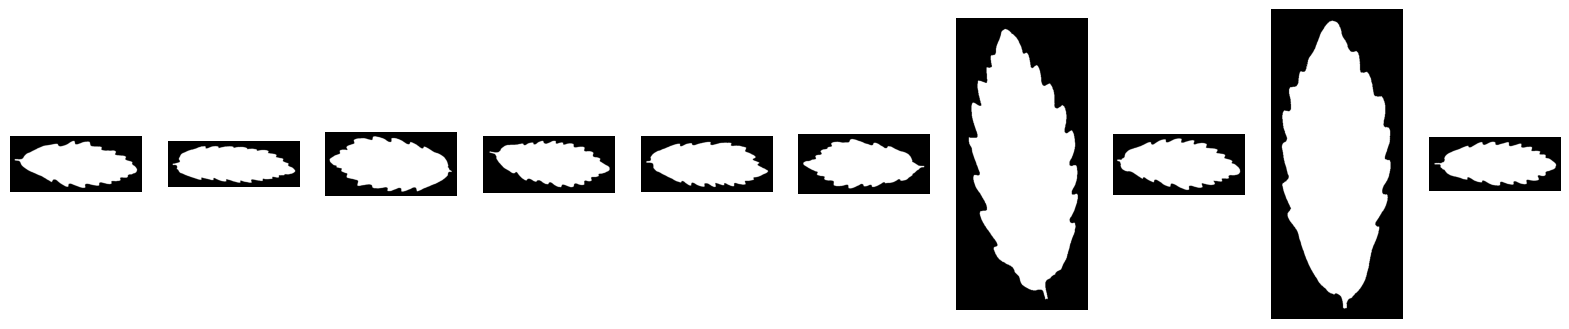
\includegraphics[width=0.9\textwidth]{img/class55_images.png}
    \caption{Exemples de classes avec des feuilles dans des orientations différentes}
\end{figure}

Également, la nature de la base de données a été un obstacle à la recherche
d'hyperparamètres. En effet, la précision des contours des feuilles étant
un critère important de différenciation des espèces, nous étions dans
l'impossibilité de compresser les images pour réduire les temps de calcul
et nous avons donc dû nous contenter de 2 modèles sur les 11 que nous
avions utilisés pour la classification sur les features.

\newpage
\section{Conclusion}
Nous sommes satisfaits des résultats obtenus, via les deux approches que nous avons
utilisées et nous sommes fiers d'avoir fait preuve d'initiative en proposant
une approche alternative de classification sur les images.

Ce projet nous a permis de mettre en pratique les connaissances acquises
durant le cours afin de comprendre les algorithmes de classification et
de choisir les paramètres à optimiser. Nous avons également pu mettre
en pratique les notions de validation croisée et de recherche d'hyperparamètres
et avons pu constater leur importance dans l'obtention de résultats satisfaisants.

\newpage
\bibliographystyle{plain}
\bibliography{references}

\end{document}